\chapter{Warum Supersymmetrie von Bedeutung sein könnte}

\lectureoverview{Vakuumfluktuationen verbinden die Themen dieses Kapitels.
Randbedingungen erzeugen die Casimir-Kraft, Schleifeneffekte gefährden die Higgs-Masse, neue virtuelle Teilchen verändern die laufenden Eichkopplungen, und die Vakuumenergie bestimmt die kosmische Expansion. Diese Probleme motivieren niedrigenergetische Supersymmetrie als Möglichkeit, die Higgs-Skala zu stabilisieren, einen Kandidaten für dunkle Materie bereitzustellen und die Vereinheitlichung der Eichkopplungen zu verbessern. Anschließend konstruieren wir Superfelder mit Grassmann-Koordinaten und verwenden die Berezin-Integration, um eine supersymmetrische Wirkung zu gewinnen.}

\section{Vakuumfluktuationen zwischen reflektierenden Platten}

Wir kehren zur Supersymmetrie zurück und klären zunächst eine Frage zum Casimir-Effekt. Man bringe zwei parallele reflektierende Platten im Abstand \(d\) an. Auch wenn keine realen Teilchen vorhanden sind, weist ein Quantenfeld Vakuumfluktuationen auf. Man kann sie sich als virtuelle Prozesse vorstellen oder gleichwertig als Nullpunktsbewegung der Oszillatormoden des Feldes. Die Platten geben Randbedingungen vor, sodass sich die erlaubten Fluktuationen zwischen ihnen von denen im unbegrenzten Raum unterscheiden.

Entscheidend ist nicht ein absoluter Energienullpunkt, sondern die Änderung, die beim Verändern des Abstands entsteht. Die Vakuumenergie pro Flächeneinheit sei \(\mathcal E(d)=E(d)/A\). Sobald \(\mathcal E\) von \(d\) abhängt, ist sie eine potenzielle Energie, und die Kraft pro Flächeneinheit beträgt
\begin{equation}
\frac{F}{A}=-\frac{d\mathcal E}{dd}.
\end{equation}
So wird aus einer Umordnung virtueller Prozesse eine beobachtbare Kraft. Im bekannten elektromagnetischen Beispiel ideal leitender Platten lauten Energie und Druck
\begin{align}
\mathcal E(d)&=-\frac{\pi^2}{720\,d^3},\\
\frac{F}{A}&=-\frac{\pi^2}{240\,d^4},
\end{align}
in den Einheiten \(\hbar=c=1\).\editorialnote{Diese Koeffizienten und die Unterscheidung zwischen der Energie pro Fläche mit Abstandsabhängigkeit \(d^{-3}\) und dem Druck mit Abstandsabhängigkeit \(d^{-4}\) klären die an der Tafel aufgeworfene Dimensionsfrage. Es handelt sich um das Standardergebnis für ideale Platten, nicht um eine hier durchgeführte Herleitung.} Das Minuszeichen steht für Anziehung.

\begin{classroomqa}
\audiencequestion{Beschreibt die vierte Potenz die Kraft oder die Energie? \lecturetimestamp{00:04:39}}
\lecturerresponse{Bei parallelen Platten in vier Raumzeitdimensionen nimmt die Energie pro Flächeneinheit wie \(d^{-3}\) ab, während die Ableitung nach \(d\) bewirkt, dass die Kraft pro Flächeneinheit wie \(d^{-4}\) abnimmt. Die Dimensionsanalyse legt diese Potenzen bereits fest, sobald \(\hbar\) und \(c\) wieder berücksichtigt werden.}
\end{classroomqa}

Man fasst die Rechnung manchmal mit der Aussage zusammen, die Platten unterbrächen virtuelle Photonenschleifen. Dieses Bild ist nützlich, solange man es nicht zu wörtlich nimmt. Die präzise Rechnung beschreibt eine Änderung des Spektrums der erlaubten Feldmoden oder gleichwertig eine Änderung der quantenwirksamen Wirkung. Beide Beschreibungen führen zur selben vom Plattenabstand abhängigen Energie.

\begin{classroomqa}
\audiencequestion{Kann die Casimir-Kraft abstoßend statt anziehend sein? \lecturetimestamp{00:07:48}}
\lecturerresponse{Ja. Das Vorzeichen ist nicht universell, sondern hängt von den Feldern, der Geometrie, den Materialien und den Randbedingungen ab. Fermionische Schleifen haben oft ein entgegengesetztes Schleifenvorzeichen als bosonische Schleifen. Das gibt der an der Tafel geäußerten Vermutung einen Anhaltspunkt, doch die fermionische Statistik allein ist kein allgemeiner Satz, dem zufolge jede Casimir-Kraft abstoßend sein muss.\editorialnote{Diese Einschränkung ersetzt eine bewusst vorläufige Antwort aus der Vorlesung durch die allgemeine Aussage, die nötig ist, um eine falsche universelle Regel zu vermeiden.}}
\end{classroomqa}

\subsection{Was wäre ein Beleg für Vakuumenergie?}

Die Casimir-Kraft wird gemessen, und auch atomare Observablen reagieren empfindlich auf Vakuumschleifen. Doch keine dieser Tatsachen belegt für sich genommen, dass eine absolute Vakuumenergie gravitiert. Ein Casimir-Experiment misst eine durch Randbedingungen verursachte Energiedifferenz; dieselbe Kraft lässt sich beschreiben, ohne einer unbeschränkten absoluten Nullpunktsumme eine operationale Bedeutung beizumessen.

Der entscheidende Test kommt aus der Gravitation. Energie ist Gravitationsladung. Wenn der leere Raum eine gleichförmige Energiedichte enthält, muss sie in die Einsteinschen Gleichungen eingehen und die kosmische Expansion beeinflussen. Die beschleunigte Expansion des Universums ist daher der direkte gravitative Beleg für eine vakuumartige Komponente.

\begin{classroomqa}
\audiencequestion{Warum bezeichnen populärwissenschaftliche Darstellungen Vakuumenergie als rätselhaft, als wüssten Physiker nicht, was sie ist? \lecturetimestamp{00:08:19}}
\lecturerresponse{Die Quantenfeldtheorie liefert für jedes Feld einen Nullpunktsbeitrag; die Möglichkeit einer Vakuumenergie ist also nicht rätselhaft. Das Rätsel ist quantitativer Art: Warum ist der gravitative Wert im Vergleich zu Schätzungen auf Grundlage bekannter Quantenfelder und eines hochenergetischen Abschneidewerts außerordentlich klein? Überraschend ist ihr nahezu vollständiges Fehlen, nicht ihr bloßes Vorhandensein.}
\end{classroomqa}

Viele Jahre lang war die beobachtungsbedingte obere Schranke so niedrig, dass es psychologisch verlockend war, die kosmologische Konstante genau auf null zu setzen und nach einem Prinzip zu suchen, das diese Auslöschung erzwingt. Präzisere kosmologische Beobachtungen ergaben stattdessen einen kleinen, von null verschiedenen Wert. Diese Entdeckung machte Vakuumenergie nicht begrifflich fremdartig; sie machte das unerklärte Ausmaß der Unterdrückung unübersehbar. Der maßgebliche Vergleich hängt von der angenommenen Ultraviolett-Skala ab, doch jede natürliche hochenergetische Schätzung verlangt eine gewaltige Auslöschung.

\section{Was eine Superladung mit einem Vielteilchenzustand macht}

Bevor wir Gründe für die Annahme von Supersymmetrie aufzählen, sollten wir ein mögliches Paradox ausräumen. Bosonen können eine Mode in beliebig großer Zahl besetzen, während eine fermionische Mode die Besetzungszahl null oder eins hat. Wenn eine Symmetrie Bosonen in Fermionen überführt, macht sie dann aus tausend Bosonen in einer Mode tausend unzulässige Fermionen?

Nein. Ein fermionischer Generator verändert jeweils ein Quant. Im Oszillatormodell sei \(a\) ein Operator, der ein Boson vernichtet, und \(c^\dagger\) ein Operator, der seinen fermionischen Partner erzeugt. Eine Superladung lässt sich darstellen als
\begin{equation}
Q=c^\dagger a.
\end{equation}
Auf einen Zustand mit \(n\) Bosonen und ohne Fermion wirkt sie folgendermaßen:
\begin{equation}
Q\ket{n,0}
=\sqrt n\,\ket{n-1,1}.
\end{equation}
Ein Boson wurde entfernt und ein Fermion hinzugefügt. Eine erneute Anwendung derselben Ladung ergibt null:
\begin{equation}
Q^2=(c^\dagger)^2a^2=0.
\end{equation}
Dies ist die Nilpotenz, die von fermionischen Erzeugungsoperatoren herrührt.

\begin{classroomqa}
\audiencequestion{Wenn viele Bosonen denselben Zustand besetzen, warum erzeugt eine Supersymmetrie-Transformation dann nicht viele Fermionen in diesem Zustand und verletzt so das Ausschließungsprinzip? \lecturetimestamp{00:12:05}}
\lecturerresponse{Der Generator ersetzt nicht die gesamte Besetzung. Er verändert den Zustand um eine Einheit der Fermionenzahl. Dieselbe fermionische Ladung lässt sich nicht wie ein gewöhnlicher Rotationsgenerator wiederholt anwenden, denn ihr Quadrat verschwindet. Eine komplementäre Ladung kann den Austausch rückgängig machen, und der gemischte Antikommutator schließt sich zur Zeittranslation.}
\end{classroomqa}

Der letzte Satz ist wesentlich. Die Kurzschreibweise \(Q^2=0\) bezieht sich auf eine einzelne chirale Komponente oder auf die einfache Ladung, die gerade angegeben wurde; sie bedeutet nicht, dass jedes Produkt von Superladungen verschwindet. In der vierdimensionalen Supersymmetrie gilt
\begin{equation}
\{Q_\alpha,\bar Q_{\dot\beta}\}
=2\sigma^\mu_{\alpha\dot\beta}P_\mu,
\end{equation}
während für die minimale Algebra ohne zentrale Ladungen
\begin{equation}
\{Q_\alpha,Q_\beta\}=0,
\qquad
\{\bar Q_{\dot\alpha},\bar Q_{\dot\beta}\}=0
\end{equation}
gilt.\editorialnote{Diese Komponentenform präzisiert die im Unterricht verwendete Kurzform, dass die wiederholte Wirkung derselben \(Q\) verschwindet, während eine Superladung und ihre konjugierte Superladung gemeinsam eine Translation erzeugen.}

\section{Drei Gründe, nach niedrigenergetischer Supersymmetrie zu suchen}

\begin{classroomqa}
\audiencequestion{Gibt es neben der Aufhebung der Vakuumenergie noch eine Motivation für Supersymmetrie? \lecturetimestamp{00:15:06}}
\lecturerresponse{Es gibt drei eng miteinander verbundene Motivationen: die Kontrolle der Higgs-Selbstenergie, ein mögliches stabiles Dunkle-Materie-Teilchen und eine deutlich genauere Annäherung der Eichkopplungen bei hohen Energien. Keine davon beweist, dass Supersymmetrie in der Natur verwirklicht ist. Zusammengenommen machen sie die Theorie jedoch zu einem ernst zu nehmenden Prüfgegenstand.}
\end{classroomqa}

Die Bezeichnung \emph{niedrigenergetische Supersymmetrie} ist relativ. Sie bedeutet nicht, dass Superpartner auf alltäglichen Skalen leicht sind, sondern dass ihre Massen nicht sehr viel höher liegen als die elektroschwache Skala und die Skalen von Beschleunigern. Alle drei Argumente verlieren an Gewicht, wenn die Superpartner beliebig weit nach oben verschoben werden.

\subsection{Die Higgs-Skala schützen}

Eine skalare Masse reagiert ungewöhnlich empfindlich auf hochenergetische Physik. Schematisch erzeugt eine bosonische Schleife eine Korrektur der Form
\begin{equation}
\delta m_H^2\big|_{\mathrm B}
\sim +\frac{\lambda}{16\pi^2}\Lambda^2,
\end{equation}
wobei \(\Lambda\) die Skala bezeichnet, bis zu der die effektive Theorie verwendet wird. Eine fermionische Schleife hat das entgegengesetzte Vorzeichen:
\begin{equation}
\delta m_H^2\big|_{\mathrm F}
\sim -\frac{|y|^2}{8\pi^2}\Lambda^2.
\end{equation}
Die Koeffizienten hängen von der Wechselwirkung und den Multiplizitäten der Felder ab. Die Supersymmetrie setzt sie jedoch zueinander in Beziehung, sodass sich die führende Ultraviolett-Empfindlichkeit zwischen den Partnern aufhebt.\editorialnote{Die schematischen Schleifenformeln zeigen die mathematische Grundlage des qualitativen Arguments zur Selbstenergie. Sie sind nicht als vollständige Berechnung der Higgs-Masse im Standardmodell gedacht.}

Das ist wichtig, weil der Erwartungswert des Higgs-Feldes die elektroschwache Skala festlegt. Die Massen von Eichbosonen und Fermionen erfüllen Beziehungen wie
\begin{equation}
m_W=\frac{gv}{2},
\qquad
m_f=\frac{y_fv}{\sqrt2}.
\end{equation}
Würde der Higgs-Sektor auf natürliche Weise auf eine enorme Skala getrieben, ginge das vertraute niederenergetische Teilchenspektrum verloren. Es sei denn, man stimmte die nackten Parameter mit äußerster Präzision gegen die radiativen Korrekturen ab.

Bei exakter Supersymmetrie wäre die Aufhebung vollständig. Exakte Supersymmetrie ist jedoch bereits durch die unterschiedlichen Massen beobachteter Bosonen und Fermionen ausgeschlossen. Bei weich gebrochener Supersymmetrie wird die quadratische Empfindlichkeit durch eine Abhängigkeit von den Aufspaltungen der Superpartner ersetzt, schematisch
\begin{equation}
\delta m_H^2
\sim
\frac{g^2}{16\pi^2}
\left(m_{\mathrm{soft}}^2-m_{\mathrm{ordinary}}^2\right)
\ln\frac{\Lambda^2}{m_{\mathrm{soft}}^2}.
\end{equation}
Die Aufhebung bleibt nur dann nützlich, wenn die Aufspaltung nicht zu groß ist.

\subsection{Ein stabiler Endpunkt für Dunkle-Materie-Kaskaden}

Teilen wir das Spektrum in gewöhnliche Teilchen und ihre Superpartner auf. Ein Fermion hat einen bosonischen Partner, ein Boson einen fermionischen Partner. Wenn die Wechselwirkungen eine Parität erhalten, die diese beiden Klassen unterscheidet, muss beim Zerfall eines Superpartners ein weiterer Superpartner übrig bleiben:
\begin{equation}
\widetilde X
\longrightarrow X+\widetilde Y
\longrightarrow X+Y+\widetilde Z
\longrightarrow\cdots.
\end{equation}
Die Kaskade kann ihren letzten Superpartner nicht abwerfen. Sie endet daher beim leichtesten supersymmetrischen Teilchen, dem LSP.

Die gebräuchliche Symmetrie ist die \(R\)-Parität:
\begin{equation}
R_p=(-1)^{3(B-L)+2s}.
\end{equation}
Teilchen des Standardmodells haben \(R_p=+1\), ihre Superpartner dagegen \(R_p=-1\). Ist \(R_p\) exakt, enthält jede Wechselwirkung eine gerade Zahl von Superpartnern, und das LSP ist stabil.\editorialnote{Supersymmetrie allein garantiert kein stabiles LSP. Seine Stabilität setzt eine erhaltene \(R\)-Parität oder eine andere Symmetrie mit derselben Konsequenz voraus; ohne sie kann das LSP zerfallen.}

Dunkle Materie muss mindestens über kosmologische Zeiträume bestehen bleiben. Außerdem muss sie schwach genug wechselwirken, um wiederholt durch die sichtbare galaktische Scheibe hindurchzutreten, ohne dabei nennenswert Energie zu verlieren. Eine elektrisch geladene oder stark wechselwirkende Teilchenpopulation würde streuen, Energie dissipieren und dazu tendieren, sich in dieselbe dünne Struktur wie gewöhnliche Materie zusammenzuziehen. Der beobachtete ausgedehnte Halo deutet dagegen auf eine neutrale, schwach wechselwirkende Komponente hin.

Damit ist das LSP nicht eindeutig bestimmt. Je nach Modell und Muster der Symmetriebrechung könnte der Kandidat eine neutrale Mischung aus elektroschwachen Eichinos und Higgsinos oder ein Gravitino sein. Geladene oder farbgeladene Kandidaten unterliegen starken Einschränkungen. Die Supersymmetrie liefert keine garantierte Antwort, sondern einen natürlichen Mechanismus für einen neutralen, langlebigen Endzustand.

\section{Laufende Kopplungen und der Hinweis auf Vereinheitlichung}

Die dritte Motivation geht von der Abschirmung der Ladung aus. Eine gemessene Kopplung hängt von der Energieskala ab, weil virtuelle Teilchen die Wechselwirkung bekleiden. Bei der Elektromagnetismus schirmt eine in einen Photonpropagator eingefügte Elektron-Positron-Schleife die Ladung auf großen Abständen ab. Bei kürzeren Abständen oder höherem Impulsübertrag liegt weniger von dieser Polarisationswolke zwischen den Sonden, und die effektive Ladung ist größer.

Schreibe
\begin{equation}
\alpha_i=\frac{g_i^2}{4\pi}.
\end{equation}
In einer Schleifenordnung verändert sich die inverse Kopplung linear mit dem Logarithmus der Energie:
\begin{equation}
\frac{d\alpha_i^{-1}}{d\ln\mu}
=-\frac{b_i}{2\pi}.
\end{equation}
Daraus folgt
\begin{equation}
\alpha_i^{-1}(\mu)
=\alpha_i^{-1}(\mu_0)
-\frac{b_i}{2\pi}\ln\frac{\mu}{\mu_0}.
\end{equation}
\editorialnote{Diese Ein-Schleifen-Gleichung ist die präzise Fassung der nahezu geraden Linien, die als Funktionen des logarithmischen Energieparameters gezeichnet werden. Schwellen und Korrekturen höherer Schleifen krümmen die Linien geringfügig.}

Oberhalb der elektroschwachen Skala lauten die drei fundamentalen Eichkopplungen
\begin{equation}
U(1)_Y,\qquad SU(2)_L,\qquad SU(3)_c.
\end{equation}
Die elektromagnetische Kopplung, die zur Anschauung bei niedrigen Energien verwendet wird, ist nach der elektroschwachen Symmetriebrechung eine Kombination der ersten beiden. In der QCD erzeugen die nichtabelschen Eichfelder eine Antischirmung: Die starke Kopplung nimmt bei kürzeren Abständen ab – das Phänomen der asymptotischen Freiheit. Daher steigt \(\alpha_3^{-1}\) mit \(\ln\mu\), während die inversen Kopplungen der anderen Wechselwirkungen andere Steigungen haben.

Die Kurven des Standardmodells nähern sich einander erkennbar an, treffen sich aber nicht in einem einzigen Punkt. Superpartner verändern die virtuellen Schleifen und damit die Koeffizienten \(b_i\). In der üblichen Normierung für große Vereinheitlichung gilt
\begin{align}
(b_1,b_2,b_3)_{\mathrm{SM}}
&=\left(\frac{41}{10},-\frac{19}{6},-7\right),\\
(b_1,b_2,b_3)_{\mathrm{MSSM}}
&=\left(\frac{33}{5},1,-3\right).
\end{align}
Bei Schwellen der Superpartner in der Nähe der TeV-Skala treffen sich die extrapolierten supersymmetrischen Kurven deutlich genauer bei ungefähr
\begin{equation}
M_{\mathrm{GUT}}\sim 10^{16}\ \mathrm{GeV}.
\end{equation}
Kein Experiment erreicht diese Skala direkt. Man misst die Kopplungen bei niedrigen Energien, bestimmt den Verlauf aus dem Feldinhalt und extrapoliert die Kurven über viele Größenordnungen. Zwei Linien schneiden sich immer irgendwo; dass drei unabhängige Linien sich nahe einem Punkt treffen, ist die nichttriviale Beobachtung.

\begin{classroomqa}
\audiencequestion{Setzt die verbesserte Extrapolation exakte Supersymmetrie und gleiche Massen der Partner voraus? \lecturetimestamp{00:38:09}}
\lecturerresponse{Nein. Supersymmetrie ist gebrochen, die Massen sind also aufgespalten. Entscheidend ist, wann die Schleifen der Superpartner in den Verlauf eingehen. Sind die Partner nicht zu schwer, ändern sich die Steigungen früh genug, damit sich die drei Kopplungen annähern. Sind sie außerordentlich schwer, setzen die supersymmetrischen Schwellen zu spät ein und die verbesserte Annäherung geht verloren.}
\end{classroomqa}

Schwellenkorrekturen und das unbekannte hochenergetische Spektrum verhindern die wörtliche Behauptung, die drei Linien träfen sich mathematisch exakt. Das Ergebnis ist dennoch bemerkenswert: Dieselbe ungefähre Skala der Superpartner, die dem Higgs-Problem hilft und einen Kandidaten für thermische Dunkle Materie liefert, verbessert auch die Vereinheitlichung.

\subsection{Gravitation und die gemeinsame hochenergetische Skala}

Die Gravitation verhält sich anders, denn ihre Ladung ist die Energie selbst. Eine nützliche dimensionslose Größe bei einer Schwerpunktsenergie \(E\) ist
\begin{equation}
\alpha_G(E)\sim GE^2
=\left(\frac{E}{M_{\mathrm{Pl}}}\right)^2.
\end{equation}
Bei gewöhnlichen Energien ist sie verschwindend klein, wächst aber quadratisch mit \(E\). Ihre Inverse nimmt daher viel schneller ab als die logarithmisch laufenden inversen Eichkopplungen und wird nahe der Planck-Skala von der Größenordnung eins.

Dieser Vergleich legt nahe, dass alle Wechselwirkungen durch benachbarte hohe Skalen bestimmt sein könnten, ist aber weniger eindeutig als die Vereinheitlichung der Eichkopplungen. Die Eichkopplungen sind dimensionslose Parameter renormierbarer Feldtheorien; die Newton-Konstante ist dimensionsbehaftet. Um die Gravitation in dasselbe Diagramm einzutragen, muss daher eine Konvention festgelegt werden.

\begin{classroomqa}
\audiencequestion{Nehmen Superpartner an denselben drei Eichwechselwirkungen teil oder definieren sie neue Kräfte? \lecturetimestamp{00:42:35}}
\lecturerresponse{Sie tragen dieselben Eichquantenzahlen wie ihre Partner. Ein Selektron hat die elektrische Ladung des Elektrons, und ein Squark trägt die entsprechende Farbe sowie die elektroschwachen Ladungen des Quarks; Spin und Masse unterscheiden sich jedoch. Ihre Schleifen verändern daher dieselben Eichwechselwirkungen, statt drei neue einzuführen.}
\end{classroomqa}

\begin{classroomqa}
\audiencequestion{Wäre die Entdeckung eines Superpartners am LHC ein endgültiger Beleg für Supersymmetrie? \lecturetimestamp{00:43:27}}
\lecturerresponse{Ein einzelnes unbekanntes Teilchen wäre nicht schon aufgrund seiner Bezeichnung ausreichend. Ein Superpartnerspektrum, das supersymmetrische Beziehungen zwischen Spins, Ladungen, Massen und Kopplungen erfüllt, wäre jedoch sehr charakteristisch. Supersymmetrie erzwingt zahlreiche miteinander verknüpfte Einschränkungen; daher wäre das detaillierte Muster der Wechselwirkungen der entscheidende Test.}
\end{classroomqa}

\subsection{Warum sich die Skala nicht folgenlos verschieben lässt}

Liegen die Superpartner nur knapp außerhalb der experimentellen Reichweite, können alle drei Motivationen weiterhin greifen. Werden ihre Massen um Größenordnungen erhöht, verschlechtert sich jedes der Argumente:
\begin{enumerate}
\item Bei der Aufhebung von Higgs-Massenkorrekturen bleibt eine große Restempfindlichkeit gegenüber der Aufspaltung.
\item Ein herkömmlicher thermischer Restbestand eines Teilchens auf der elektroschwachen Skala entsteht nicht mehr bei der erwarteten Skala.
\item Die Schwellen im Verlauf der Eichkopplungen verschieben sich nach oben, und die drei Kopplungen treffen sich weniger genau.
\end{enumerate}
Supersymmetrie könnte weiterhin auf einer viel höheren Skala existieren, würde diese bestimmten niederenergetischen Probleme dann aber nicht mehr auf dieselbe ökonomische Weise lösen. Dass die Idee sich lange gehalten hat, ist kein Beleg dafür, dass die Natur sie verwirklichen muss; es zeigt, dass der Vorschlag in sich schlüssig genug ist, um einen entscheidenden Test zu verdienen.

\section{Was die Kosmologie über dunkle Materie aussagen kann und was nicht}

\begin{classroomqa}
\audiencequestion{Kann die Standardkosmologie die Menge dunkler Materie und die Masse jedes Dunkle-Materie-Teilchens bestimmen, ähnlich wie die Nukleosynthese den Wasserstoff- und Heliumanteil einschränkt? \lecturetimestamp{00:46:32}}
\lecturerresponse{Die Kosmologie misst die gesamte Massendichte dunkler Materie sehr genau, doch aus der Dichte allein lassen sich Masse und Anzahl nicht voneinander trennen. Dieselbe Dichte könnte von wenigen schweren Teilchen oder einer enormen Anzahl sehr leichter Teilchen getragen werden. Um das mikroskopische Teilchen zu identifizieren, braucht es zusätzliche Theorie oder nichtgravitative Beobachtungen.}
\end{classroomqa}

Zwei grundlegende Möglichkeiten veranschaulichen diese Mehrdeutigkeit. Ein schwach wechselwirkendes Teilchen nahe der elektroschwachen Skala oder der TeV-Skala kann aus einem heißen thermischen Bad ausfrieren. Am anderen Ende des Spektrums kann ein extrem leichtes Boson wie ein Axion eine kohärente Feldkonfiguration oder ein Kondensat bilden. Zwischenliegende Möglichkeiten sind nicht allein deshalb ausgeschlossen, weil die beiden am besten entwickelten Mechanismen nahe den entgegengesetzten Enden liegen.

Die Struktur des Halos liefert selbst eine wichtige Einschränkung. Dunkle Materie durchquert gewöhnliche Materie nahezu reibungsfrei und bleibt daher räumlich ausgedehnt, statt zu einer leuchtenden Scheibe zusammenzufallen. Rotationskurven und andere gravitative Phänomene zeigen, dass die Masse vorhanden ist, zählen aber für sich genommen nicht die Teilchen.

\begin{classroomqa}
\audiencequestion{Könnte das frühe Universum anfangs nur Superteilchen enthalten haben, die später zu den Teilchen zerfielen, die wir beobachten? \lecturetimestamp{00:49:11}}
\lecturerresponse{Bei Temperaturen, die weit über allen relevanten Massen liegen, bringen schnelle Reaktionen die Teilchenarten in Richtung eines thermischen Gleichgewichts, statt eine beliebige einseitige Besetzung zu erhalten. Gewöhnliche Stöße erzeugen Superpartner, wenn diese unterrepräsentiert sind; Stöße und Zerfälle von Superpartnern führen demgegenüber gewöhnliche Teilchen wieder zu. Die genaue Häufigkeit hängt von den Wechselwirkungen und den Freiheitsgraden ab, doch das heiße Plasma strebt fortwährend einem Gleichgewicht entgegen.}
\end{classroomqa}

Während das Universum abkühlt, werden massive Teilchenarten exponentiell unterdrückt und annihilieren oder zerfallen. Ein stabiles LSP folgt dem Gleichgewicht nicht mehr, sobald seine Wechselwirkungsrate langsamer als die kosmische Expansion wird:
\begin{equation}
\Gamma_{\mathrm{ann}}
\sim n\langle\sigma v\rangle
\lesssim H.
\end{equation}
Die verbleibenden Teilchen bilden einen Restbestand.\editorialnote{Dieses Ausfrierkriterium ist die übliche quantitative Ergänzung des Arguments zum thermischen Gleichgewicht. Andere LSP-Kandidaten, insbesondere sehr schwach gekoppelte Gravitinos, können eine nichtthermische Entwicklung durchlaufen.}

\begin{classroomqa}
\audiencequestion{Zu welchem gewöhnlichen Teilchen ist das LSP der Partner, und muss es nichtwechselwirkend sein? \lecturetimestamp{00:51:05}}
\lecturerresponse{Darauf gibt es keine modellunabhängige Antwort. Von einem geeigneten LSP für dunkle Materie erwartet man, dass es elektrisch neutral und farblos ist, aber es muss nicht vollständig nichtwechselwirkend sein. Es kann sich um eine Mischung handeln, die mit dem Photon, den schwachen Eichbosonen und den Higgs-Feldern zusammenhängt, oder um ein Gravitino. Seine genaue Identität ergibt sich aus dem Spektrum der Supersymmetriebrechung.}
\end{classroomqa}

\section{Vakuumdiagramme, Selbstenergiediagramme und Expansion}

\begin{classroomqa}
\audiencequestion{Was ist der Unterschied zwischen der Higgs-Divergenz und der Vakuumenergiedivergenz? \lecturetimestamp{00:52:09}}
\lecturerresponse{Ein Vakuumdiagramm hat keine äußeren Teilchenlinien. Es verändert die effektive Wirkung des leeren Raums und trägt zur Vakuumenergie bei. Ein Higgs-Selbstenergiediagramm hat zwei äußere Higgs-Beine. Es verändert den Higgs-Propagator und damit dessen Masse. Beide beinhalten virtuelle Fluktuationen, beantworten aber unterschiedliche Fragen.}
\end{classroomqa}

Man kann sich ein reales Teilchen als Störung vorstellen, die in das Vakuum eingebracht wird. Vakuumfluktuationen, die an diese Störung ankoppeln, verschieben ihre Ausbreitung und Masse. Auch Casimir-Platten verändern Vakuumfluktuationen, allerdings durch makroskopische Randbedingungen. Gemeinsam ist allen Fällen, dass Quantenfluktuationen auf etwas Eingebrachtes reagieren; welche beobachtbare Größe korrigiert wird, ist jeweils verschieden.

\vspace{-2pt}\subsection{Materie, Strahlung und Vakuum verdünnen sich unterschiedlich}

Sei \(a(t)\) der kosmologische Skalenfaktor und
\begin{equation}
H=\frac{\dot a}{a}
\end{equation}
der Hubble-Parameter. Aus der lokalen Energie-Impuls-Erhaltung in einem homogenen Universum folgt
\begin{equation}
\dot\rho+3H(\rho+p)=0.
\end{equation}
Für eine Zustandsgleichung \(p=w\rho\) ergibt sich durch Integration
\begin{equation}
\rho(a)\propto a^{-3(1+w)}.
\end{equation}
\editorialnote{Die Kontinuitätsgleichung liefert die kompakte Herleitung, die den Erklärungen anhand der Teilchenzählung und der Wellenlängendehnung zugrunde liegt.}

Für kalte, nichtrelativistische Materie gilt \(p\approx0\), also
\begin{equation}
\rho_m\propto a^{-3}.
\end{equation}
Ein festes komobiles Volumen wächst wie \(a^3\), während die von seinen Teilchen getragene Ruheenergie näherungsweise konstant bleibt.

Für Strahlung gilt \(p=\rho/3\) und damit
\begin{equation}
\rho_r\propto a^{-4}.
\end{equation}
Drei Potenzen stammen aus der Verdünnung der Teilchenzahldichte. Die vierte kommt von der Rotverschiebung:
\begin{equation}
\lambda\propto a,
\qquad
E_\gamma=\frac{2\pi\hbar c}{\lambda}\propto a^{-1}.
\end{equation}

\begin{classroomqa}
\audiencequestion{Wenn ein Photon eine Wellenfunktion hat, warum können wir es bei der Herleitung des Verdünnungsgesetzes als Teilchen statt als Welle beschreiben? \lecturetimestamp{00:58:21}}
\lecturerresponse{Die Unterscheidung ändert nichts an der Skalierung. In der Teilchenbeschreibung bleibt die Anzahl in einem komobilen Volumen konstant, und jedes Quant wird gemäß \(a^{-1}\) rotverschoben. In der Beschreibung mit klassischen Wellen dehnt sich die Wellenlänge aus, und die Feldenergie nimmt um denselben Betrag ab. Wir können jeweils die Beschreibung verwenden, mit der sich die Expansion am einfachsten veranschaulichen lässt.}
\end{classroomqa}

Für Vakuumenergie gilt \(p_\Lambda=-\rho_\Lambda\), also
\begin{equation}
\rho_\Lambda=\text{constant}.
\end{equation}
Sie wird durch die Expansion des Raums nicht verdünnt. Ein komobiles Gebiet enthält tatsächlich
\begin{equation}
E_\Lambda=\rho_\Lambda a^3V_0,
\end{equation}
und dieser Wert wächst mit seinem physikalischen Volumen. Daraus ergibt sich die Frage nach der Energieerhaltung, auf die wir gleich eingehen.

Die unterschiedlichen Potenzen ordnen die kosmische Entwicklung. Strahlung nimmt am schnellsten ab, Materie langsamer, und Vakuumenergie überhaupt nicht. Daher kann ein kleiner Vakuumterm im frühen Universum vernachlässigbar sein und zu späten Zeiten dominieren. Mit den hier besprochenen groben Werten entfallen gegenwärtig etwa \(70\%\) auf Vakuumenergie und \(30\%\) auf Materie; der Strahlungsanteil ist deutlich kleiner.

\section{Geometrie ist gleich Energie}

Die Zeit-Zeit-Komponente der Einsteinschen Gleichungen macht aus den vorherigen Skalierungsgesetzen eine Dynamik. Die Tafel beginnt mit einem Merksatz und einem einzigen geometrischen Term.

\begin{figure}[H]\centering
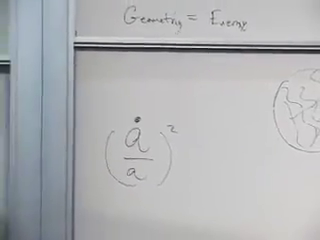
\includegraphics[width=0.68\textwidth]{lecture_06_figure_03.png}\lectureframe{01:06:37.088}\caption{Der leitende Merksatz \emph{Geometrie ist gleich Energie}, darunter steht der Expansionsterm \(H^2=(\dot a/a)^2\).}\end{figure}

Für ein homogenes und isotropes Universum lautet die erste Friedmann-Gleichung
\begin{equation}
H^2+\frac{k}{a^2}
=\frac{8\pi G}{3}\rho,
\end{equation}
in den Einheiten \(c=1\), wobei \(k=+1,0,-1\) für geschlossene, flache beziehungsweise offene räumliche Geometrie steht, und
\begin{equation}
\rho
=\rho_{\mathrm{ordinary}}
+\rho_{\mathrm{dark}}
+\rho_{\mathrm{radiation}}
+\rho_{\mathrm{vacuum}}.
\end{equation}
Das neben \(1/a^2\) sichtbare Vorzeichen hängt davon ab, ob der Krümmungsterm auf der linken Seite bleibt oder auf die rechte Seite gebracht wird, sowie vom Wert von \(k\).

\begin{figure}[H]\centering
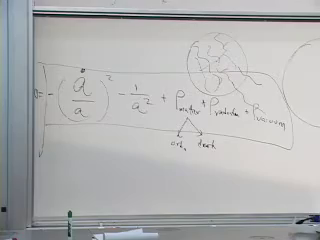
\includegraphics[width=0.96\textwidth]{lecture_06_figure_04.png}\lectureframe{01:08:46.794}\caption{Die vollständige Bilanz an der Tafel: Expansion und räumliche Krümmung auf der geometrischen Seite, Materie, Strahlung und Vakuumenergie auf der Quellenseite. Die Materie wird weiter in gewöhnliche und dunkle Komponenten aufgeteilt.}\end{figure}

\subsection{Die kosmologische Hamiltonsche Nebenbedingung}

\begin{classroomqa}
\audiencequestion{Wenn die Vakuumenergie in einem komobilen Gebiet mit der Expansion des Universums wächst, gibt es dann eine konstante Nettoenergiedichte oder eine erhaltene Gesamtenergie? \lecturetimestamp{01:01:51}}
\lecturerresponse{Die allgemeine Relativitätstheorie liefert keine universelle globale Energie für eine beliebige expandierende Raumzeit. In der homogenen kosmologischen Reduktion ist die Zeit-Zeit-Einsteingleichung jedoch eine Hamiltonsche Nebenbedingung. Bringt man Geometrie und Materie auf eine Seite, verschwindet der eingeschränkte Hamiltonoperator. Die veränderlichen Materieterme werden durch die gravitativen Freiheitsgrade ausgeglichen und nicht durch eine gewöhnliche, in einer Kiste eingeschlossene konstante Energie.}
\end{classroomqa}

Schematisch lautet die kanonische Aussage
\begin{equation}
\mathcal H_{\mathrm{gravity}}
+\mathcal H_{\mathrm{matter}}
=0.
\end{equation}
Dies ist die präzise Bedeutung der Aussage, dass die Gesamtenergie null ist. Es handelt sich um eine durch die Invarianz unter Umparametrisierungen der Zeit erzwungene Bewegungsgleichung, nicht um die Behauptung, dass jede lokale Energiedichte verschwindet. In einem komovierenden Volumen bleibt die Energie gewöhnlicher Materie ungefähr konstant, die Strahlungsenergie nimmt ab und die Vakuumenergie wächst; zugleich passen sich der gravitative Beitrag und die Expansionsrate so an, dass Einsteins Zwangsbedingung erfüllt bleibt.

Die lokale Erhaltung gilt weiterhin exakt:
\begin{equation}
\nabla_\mu T^{\mu\nu}=0.
\end{equation}
Für das homogene Fluid ist dies genau die Kontinuitätsgleichung
\(\dot\rho+3H(\rho+p)=0\). Was im Allgemeinen nicht gilt, ist die aus der flachen Raumzeit vertraute Vorstellung, dass es in einem expandierenden Universum zusätzlich eine einzige koordinatenunabhängige globale Summe der Materieenergie geben müsse, die erhalten bleibt.\editorialnote{Diese Unterscheidung präzisiert die Aussage im Unterricht, die Energie sei immer null: Die lokale kovariante Erhaltung und die kosmologische Hamilton-Zwangsbedingung gelten exakt, während eine eindeutige globale Energie aus Materie und Gravitation im Allgemeinen nicht definiert ist.}

\begin{classroomqa}
\audiencequestion{Ist die Null-Zwangsbedingung ausschlaggebend dafür, ob das Universum offen, geschlossen oder flach ist? \lecturetimestamp{01:04:42}}
\lecturerresponse{Nein. Die Hamilton-Zwangsbedingung gilt in allen Fällen. Offene, flache und geschlossene Universen unterscheiden sich durch das Krümmungskennzeichen \(k\) und damit durch den Term \(k/a^2\). Die Krümmung verändert einen Beitrag zur Bilanz; sie setzt die Zwangsbedingung weder in Kraft noch außer Kraft.}
\end{classroomqa}

\section{Grassmann-Koordinaten und Superfelder}

\begin{classroomqa}
\audiencequestion{Kommen Grassmann-Zahlen tatsächlich in der Lagrange-Funktion der Theorie vor? \lecturetimestamp{01:09:37}}
\lecturerresponse{Sie treten zunächst auf, weil Fermionfelder Grassmann-ungerade sind. Außerdem treten sie als Koordinaten des Superspace auf. Superfelder hängen von diesen ungeraden Koordinaten ab, und supersymmetrische Wirkungen werden durch Ableiten und Integrieren nach ihnen gebildet.}
\end{classroomqa}

Ein gewöhnliches Feld ist eine Funktion der Raumzeit,
\begin{equation}
\phi=\phi(x^\mu).
\end{equation}
Die minimale Supersymmetrie in vier Dimensionen erweitert \(x^\mu\) um einen zweikomponentigen ungeraden Spinor \(\theta^\alpha\) und seinen konjugierten Spinor \(\bar\theta^{\dot\alpha}\):
\begin{equation}
z^M=(x^\mu,\theta^\alpha,\bar\theta^{\dot\alpha}).
\end{equation}
Es gibt zwei komplexe ungerade Komponenten oder vier reelle ungerade Richtungen. Ein Superfeld ist eine Funktion auf diesem Superspace:
\begin{equation}
\Phi=\Phi(x,\theta,\bar\theta).
\end{equation}

Dies sind keine winzigen räumlichen Dimensionen im Sinne der Metrik. Eine Grassmann-Koordinate hat keinen positiven numerischen Betrag. Sie als klein zu bezeichnen, dient als Merkhilfe für ihre Nilpotenz:
\begin{equation}
(\theta^\alpha)^2=0,
\qquad
\theta^\alpha\theta^\beta=-\theta^\beta\theta^\alpha.
\end{equation}
\editorialnote{Der Grund dafür, dass jede Entwicklung in endlich vielen Grassmann-Koordinaten abbricht, ist die Nilpotenz, nicht numerische Kleinheit.}

Bei vier unabhängigen ungeraden Koordinaten hat ein vollständig allgemeines Superfeld höchstens \(2^4=16\) Grassmann-Monomiale. Schematisch gilt:
\begin{equation}
\begin{aligned}
\Phi(x,\Theta)={}&\phi(x)+\Theta_A\psi_A(x)\\
&+\frac{1}{2}\Theta_A\Theta_B Z_{AB}(x)+\cdots\\
&+\Theta_1\Theta_2\Theta_3\Theta_4D(x),
\end{aligned}
\end{equation}
wobei \(\Theta_A\) zusammenfassend für die vier reellen ungeraden Koordinaten steht. Da das gesamte Superfeld als gerade gewählt werden kann, sind die Koeffizienten gerader Potenzen bosonisch und die Koeffizienten ungerader Potenzen fermionisch. Ein einziges Superfeld bündelt somit ein endliches Multiplett gewöhnlicher Komponentenfelder.

Diese Bündelung ist mehr als bloße Notation. Die Supersymmetrie wirkt geometrisch als Verschiebung in den ungeraden Richtungen, verbunden mit einer Raumzeitverschiebung. Eine nach den Regeln des Superspace aus Superfeldern konstruierte Lagrange-Funktion besitzt die Symmetrie ebenso, wie eine aus Tensoren konstruierte skalare Lagrange-Funktion Rotations- oder Lorentz-Invarianz besitzt.

Die Wirkung enthält nun Grassmann-Maße. Ein typischer Term über den gesamten Superspace hat die Form
\begin{equation}
S_D=\int d^4x\,d^2\theta\,d^2\bar\theta\,
\mathcal K(\Phi,\Phi^\dagger).
\end{equation}
Chirale Terme verwenden stattdessen
\begin{equation}
S_F=\int d^4x\,d^2\theta\,W(\Phi)+\mathrm{h.c.}
\end{equation}
\editorialnote{Die Unterscheidung zwischen Maßen über den gesamten Superspace und chiralen Maßen ist die übliche Präzisierung der schematischen \(d^4x\,d^4\theta\)-Wirkung. An konkreten Beispielen wird sich zeigen, welches Maß jeweils geeignet ist.}

Damit sind wir bei einer Frage angelangt, die sich mit gewöhnlicher Analysis nicht beantworten lässt: Was bedeutet die Integration über eine antikommutierende Koordinate?

\section{Berezin-Integration}

\subsection{Das gewöhnliche Vorbild: eine totale Ableitung}

Betrachten wir zunächst eine gewöhnliche Funktion \(F(x)\), die für große positive und negative Werte von \(x\) gegen null geht. Der Hauptsatz der Differential- und Integralrechnung liefert
\begin{equation}
\int_{-\infty}^{\infty}dx\,\frac{dF}{dx}
=F(\infty)-F(-\infty)
=0.
\end{equation}

\begin{figure}[H]
\centering
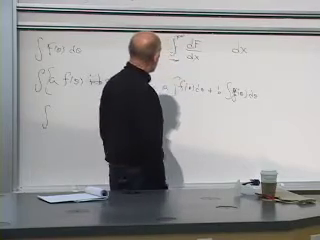
\includegraphics[width=0.88\textwidth]{lecture_06_figure_05.png}
\lectureframe{01:26:31.594}
\caption{Das gewöhnliche Vorbild für die Berezin-Integration: Das Integral einer totalen Ableitung lässt sich auf Randwerte zurückführen und verschwindet, wenn die Funktion im Unendlichen gegen null geht. Die untere Zeile an der Tafel ist teilweise verdeckt; deshalb wird die Gleichung im Text vollständig angegeben.}
\end{figure}

Wir wollen, dass das Grassmann-Integral linear ist und die nützliche Eigenschaft teilt, dass das Integral einer totalen Ableitung null ergibt. Für eine ungerade Koordinate fordern wir
\begin{align}
\int d\theta\,[af(\theta)+bg(\theta)]
&=
a\int d\theta\,f(\theta)
+b\int d\theta\,g(\theta),\\
\int d\theta\,\partial_\theta f(\theta)&=0.
\end{align}
Die zweite Bedingung ist das algebraische Analogon zur Translationsinvarianz des Maßes. Es gibt weder Randpunkte einer Zahlengeraden mit ungerader Koordinate noch eine Summe über winzige Intervalle.

\begin{classroomqa}
\audiencequestion{Geben wir die Vorstellung auf, Integration sei die Umkehroperation der Differentiation, wenn es kein unbestimmtes Grassmann-Integral gibt? \lecturetimestamp{01:21:19}}
\lecturerresponse{Ja. Die Berezin-Integration ist ein bestimmtes lineares Funktional, keine Stammfunktion. Für eine Grassmann-Variable wird sie tatsächlich durch dieselbe algebraische Operation wie die Differentiation dargestellt.}
\end{classroomqa}

\begin{classroomqa}
\audiencequestion{Ist auch die \(d^4x\)-Integration über die gesamte Raumzeit ein bestimmtes Integral? \lecturetimestamp{01:21:34}}
\lecturerresponse{Ja. Bei der Integration der Wirkung über die Raumzeit werden Randbedingungen vorausgesetzt. Der Unterschied besteht darin, dass sich gewöhnliche Raumzeitintegration als Grenzwert von Summen verstehen lässt, während Grassmann-Integration algebraisch durch ihre Wirkung auf die endliche Basis \(1,\theta\) definiert ist.}
\end{classroomqa}

\subsection{Eine Variable}

Jede Funktion einer ungeraden Variable lässt sich schreiben, wobei ihr Koeffizient in der festgelegten Reihenfolge rechts steht:
\begin{equation}
f(\theta)=a+\theta b.
\end{equation}
Da \(\partial_\theta\theta=1\) gilt, folgt aus der Regel für totale Ableitungen
\begin{equation}
\int d\theta\,1=0.
\end{equation}
Die verbleibende Normierung wird so gewählt, dass
\begin{equation}
\int d\theta\,\theta=1.
\end{equation}
Folglich gilt:
\begin{equation}
\int d\theta\,f(\theta)=b.
\end{equation}
Das Integral extrahiert den Koeffizienten der höchsten verfügbaren Potenz. Bei der hier verwendeten Konvention der Linksableitung gilt
\begin{equation}
\partial_\theta f=b
=\int d\theta\,f.
\end{equation}

\begin{classroomqa}
\audiencequestion{Gibt es eine Funktion \(F(\theta)\), für die \(\partial_\theta F=\theta\) gilt? \lecturetimestamp{01:30:05}}
\lecturerresponse{Nein. Eine solche Funktion müsste einen Term proportional zu \(\theta^2\) enthalten, aber \(\theta^2=0\). Auch daran sieht man, warum es kein Grassmann-Analogon einer unbestimmten Stammfunktion gibt.}
\end{classroomqa}

\subsection{Zwei Variablen und die Reihenfolge des Maßes}

Für ein komplexes Paar \(\theta,\bar\theta\) schreiben wir eine allgemeine gerade Funktion in der geordneten Form
\begin{equation}
f(\theta,\bar\theta)
=a+\bar\theta\psi+\bar\psi\theta+b\,\bar\theta\theta.
\end{equation}
Einen höheren Term gibt es nicht, denn
\begin{equation}
\theta^2=\bar\theta^2=0,
\qquad
\bar\theta\theta=-\theta\bar\theta.
\end{equation}

Wir legen nun die Konvention fest:
\begin{equation}
\int d\theta\,d\bar\theta\,
\bar\theta\theta=1.
\end{equation}
Bei iterierten Integralen wirkt die benachbarte Operation \(d\bar\theta\) zuerst. Damit ergibt sich folgende Tabelle:
\begin{align}
\int d\theta\,d\bar\theta\,1&=0,\\
\int d\theta\,d\bar\theta\,\theta&=0,\\
\int d\theta\,d\bar\theta\,\bar\theta&=0,\\
\int d\theta\,d\bar\theta\,\bar\theta\theta&=1.
\end{align}
Somit gilt:
\begin{equation}
\int d\theta\,d\bar\theta\,
f(\theta,\bar\theta)=b.
\end{equation}

\begin{classroomqa}
\audiencequestion{Ist es bei einem linearen Term in \(\theta\) tatsächlich die Integration nach \(\theta\), die das Doppelintegral verschwinden lässt? \lecturetimestamp{01:34:59}}
\lecturerresponse{Nein; in der mündlichen Erklärung waren die Rollen vertauscht. Die Integration nach \(\theta\) bezüglich \(\theta\) ergibt eins. Das Ergebnis enthält dann kein \(\bar\theta\) mehr, und das verbleibende Integral von eins nach \(\bar\theta\) verschwindet. In jedem Fall bleibt ein Doppelintegral nur dann übrig, wenn beide Variablen vorkommen.}
\end{classroomqa}

\begin{classroomqa}
\audiencequestion{Ändert sich das Vorzeichen des Integrals, wenn \(\theta\) und \(\bar\theta\) vertauscht werden? \lecturetimestamp{01:36:33}}
\lecturerresponse{Ja. Ungerade Variablen und ungerade Maße antikommutieren. Mit der obigen Konvention gilt
\[
\int d\bar\theta\,d\theta\,\bar\theta\theta=-1.
\]
Man muss daher eine Reihenfolge festlegen und konsequent beibehalten. Die Physik ist unabhängig von der Konvention, die Zwischenschritte sind es jedoch nicht.}
\end{classroomqa}

Für \(n\) unabhängige Grassmann-Variablen ergibt sich unmittelbar folgendes Muster:
\begin{equation}
\int d\theta_n\cdots d\theta_1\,
f(\theta_1,\ldots,\theta_n)
\end{equation}
extrahiert den Koeffizienten des geordneten Monomials höchsten Grades
\(\theta_1\cdots\theta_n\), bis auf das durch die gewählte Reihenfolge der Variablen und Maße festgelegte Vorzeichen. Diese einfache Regel zur Extraktion von Komponenten ist das Herzstück der Wirkungen im Superspace. Eine Supersymmetrie-Variation wird zu einer ungeraden totalen Ableitung, die das Superspace-Integral verwirft, so wie eine gewöhnliche Wirkung unter geeigneten Randbedingungen eine totale Ableitung bezüglich der Raumzeit verwirft.

\section{Warum ein so einfacher Kalkül so viel bewirkt}

Die Regeln wirken nahezu trivial:
\begin{equation}
\int d\theta\,1=0,
\qquad
\int d\theta\,\theta=1.
\end{equation}
Doch mit ihnen lassen sich wechselwirkende Feldtheorien aufbauen, in denen Beziehungen zwischen bosonischen und fermionischen Massen und Kopplungen automatisch erhalten bleiben. Der Zweck des Superspace-Kalküls entspricht dem des Tensor-Kalküls in der Relativitätstheorie: Die Notation wird so eingerichtet, dass die gewünschte Symmetrie jede zulässige Umformung übersteht.

Die Vorzeichenbuchhaltung ist der Preis dafür. Jeder Tausch zweier ungerader Objekte liefert ein Minuszeichen, und eine Rechnung kann konzeptionell richtig sein und dennoch an einer einzigen falschen Reihenfolge scheitern. Diese Schwierigkeit ist kein Beiwerk, sondern der algebraische Ausdruck der fermionischen Statistik.

\begin{classroomqa}
\audiencequestion{Wurden Grassmann-Zahlen zusammen mit der Supersymmetrie erfunden, oder gab es sie schon vorher? \lecturetimestamp{01:41:19}}
\lecturerresponse{Sie sind viel älter. Hermann Grassmann entwickelte die zugrunde liegende äußere Algebra im neunzehnten Jahrhundert. Differentialformen verwenden bereits antikommutierende Basiselemente; die Quantenfeldtheorie und die Supersymmetrie des zwanzigsten Jahrhunderts gaben derselben Mathematik eine neue physikalische Rolle.}
\end{classroomqa}

Nun können wir uns konkreten Konstruktionen zuwenden. Superfelder bündeln vollständige Boson-Fermion-Multipletts, Superspace-Ableitungen erhalten die Algebra, und die Berezin-Integration extrahiert die Komponentenwirkung. Als Nächstes wenden wir diesen Formalismus auf das einfachste eindimensionale Modell an und übertragen ihn anschließend auf die Feldtheorie.
